\documentclass{article}

\usepackage[utf8]{inputenc}
\usepackage[english]{babel}

\usepackage{amsmath,amsfonts,amssymb}
\usepackage{fullpage}
\usepackage{verbatim}

\usepackage{tikz,pgfplots}

\pgfplotsset{
    width=160mm,height=150mm,
    major grid style={thin,dotted,color=black!50},
    minor grid style={thin,dotted,color=black!50},
    grid,
    every axis/.append style={
        line width=0.5pt,
        tick style={
            line cap=round,
            thin,
            major tick length=4pt,
            minor tick length=2pt,
        },
    },
    legend cell align=left,
    legend pos=north west,
}

%%%%%%%%%%%%%%%%%%%%%%%%%%%%%%%%%%%%%%%%%%%%%%%%%%%%%%%%%%%%%%%%%%%%%%%%%%%%%%%%

\begin{document}

\section{Construction times and memory utilization}
% IMPORT-DATA stats sqlplot.txt

\begin{center}
    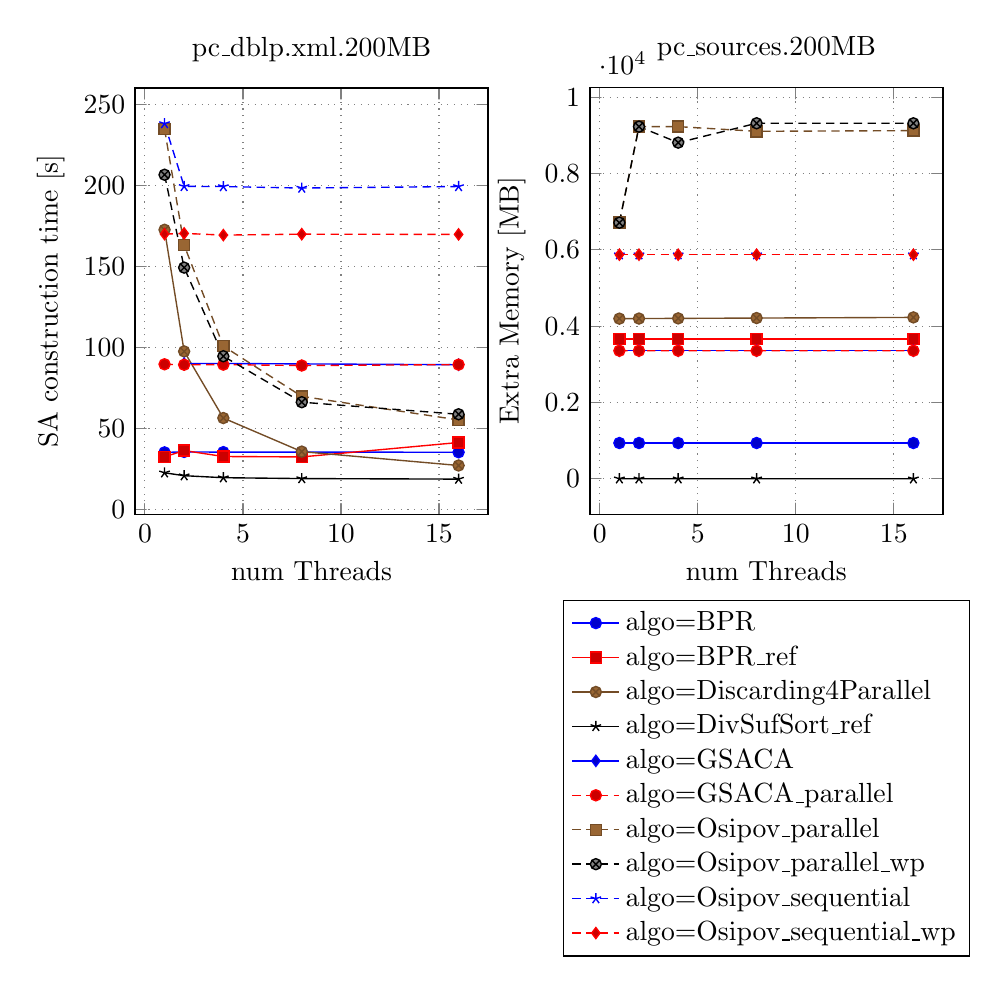
\begin{tikzpicture}
        \begin{axis}[
                name=axis1,
                width=0.5\textwidth,
                height=70mm,
                title={pc\_dblp.xml.200MB},
                xlabel={num Threads},
                ylabel={SA construction time [s]},
            ]

            %% MULTIPLOT(algo) SELECT threads AS x, time/1000 AS y, MULTIPLOT
            %% FROM stats WHERE rep_i=0 AND input="pc_dblp.xml.200MB" AND NOT algo="Deep-Shallow_par" GROUP BY MULTIPLOT,x ORDER BY MULTIPLOT,x
            \addplot coordinates { (1,35.0587) (2,35.3393) (4,35.2042) (8,35.2424) (16,35.1312) };
            \addlegendentry{algo=BPR};
            \addplot coordinates { (1,32.3077) (2,36.1792) (4,32.5017) (8,32.2455) (16,41.1532) };
            \addlegendentry{algo=BPR\_ref};
            \addplot coordinates { (1,172.585) (2,97.4388) (4,56.2671) (8,35.5243) (16,26.9513) };
            \addlegendentry{algo=Discarding4Parallel};
            \addplot coordinates { (1,22.4336) (2,20.6522) (4,19.4098) (8,18.8698) (16,18.539) };
            \addlegendentry{algo=DivSufSort\_ref};
            \addplot coordinates { (2,89.9371) (4,89.9752) (16,89.205) };
            \addlegendentry{algo=GSACA};
            \addplot coordinates { (1,89.4786) (2,89.1937) (4,89.2681) (8,88.7186) (16,89.2647) };
            \addlegendentry{algo=GSACA\_parallel};
            \addplot coordinates { (1,234.873) (2,163.015) (4,100.693) (8,69.6718) (16,55.088) };
            \addlegendentry{algo=Osipov\_parallel};
            \addplot coordinates { (1,206.596) (2,149.208) (4,94.4544) (8,66.0576) (16,58.6044) };
            \addlegendentry{algo=Osipov\_parallel\_wp};
            \addplot coordinates { (1,238.201) (2,199.39) (4,199.285) (8,198.365) (16,199.305) };
            \addlegendentry{algo=Osipov\_sequential};
            \addplot coordinates { (1,169.915) (2,170.341) (4,169.297) (8,169.868) (16,169.725) };
            \addlegendentry{algo=Osipov\_sequential\_wp};

            \legend{}
        \end{axis}
        \begin{axis}[
                at={(axis1.outer north east)},
                anchor=outer north west,
                name=axis2,
                width=0.5\textwidth,
                height=70mm,
                title={pc\_sources.200MB},
                xlabel={num Threads},
                ylabel={Extra Memory [MB]},
                legend style={at={(0.5, -0.2)}, anchor=north},
            ]

            %% MULTIPLOT(algo) SELECT threads AS x, memPeak/1000000 AS y, MULTIPLOT
            %% FROM (
            %% SELECT algo, input, MEDIAN(memFinal) AS memFinal, MEDIAN(memOff) AS memOff, AVG(memPeak) AS memPeak, prefix, rep, threads, MEDIAN(time) AS time FROM stats GROUP BY algo, input, prefix, rep, threads
            %% ) WHERE input="pc_sources.200MB" AND NOT algo="Deep-Shallow_par" GROUP BY MULTIPLOT,x ORDER BY MULTIPLOT,x
            \addplot coordinates { (1,937.472) (2,937.472) (4,937.472) (8,937.472) (16,937.472) };
            \addlegendentry{algo=BPR};
            \addplot coordinates { (1,3662.5) (2,3662.5) (4,3662.5) (8,3662.5) (16,3662.5) };
            \addlegendentry{algo=BPR\_ref};
            \addplot coordinates { (1,4196.45) (2,4198.69) (4,4202.98) (8,4211.56) (16,4228.68) };
            \addlegendentry{algo=Discarding4Parallel};
            \addplot coordinates { (1,0.264792) (2,0.264029) (4,0.264573) (8,0.265661) (16,0.267837) };
            \addlegendentry{algo=DivSufSort\_ref};
            \addplot coordinates { (1,3355.45) (2,3355.45) (4,3355.45) (8,3355.45) (16,3355.45) };
            \addlegendentry{algo=GSACA};
            \addplot coordinates { (1,3355.45) (2,3355.45) (4,3355.46) (8,3355.46) (16,3355.48) };
            \addlegendentry{algo=GSACA\_parallel};
            \addplot coordinates { (1,6710.71) (2,9227.11) (4,9227.11) (8,9104.85) (16,9122.25) };
            \addlegendentry{algo=Osipov\_parallel};
            \addplot coordinates { (1,6710.71) (2,9227.11) (4,8807.71) (8,9315.62) (16,9314.56) };
            \addlegendentry{algo=Osipov\_parallel\_wp};
            \addplot coordinates { (1,5871.84) (2,5871.84) (4,5871.84) (8,5871.84) (16,5871.84) };
            \addlegendentry{algo=Osipov\_sequential};
            \addplot coordinates { (1,5871.84) (2,5871.84) (4,5871.84) (8,5871.84) (16,5871.84) };
            \addlegendentry{algo=Osipov\_sequential\_wp};

        \end{axis}
    \end{tikzpicture}
\end{center}

\section{Example: 4 plots aligned}
\begin{center}
    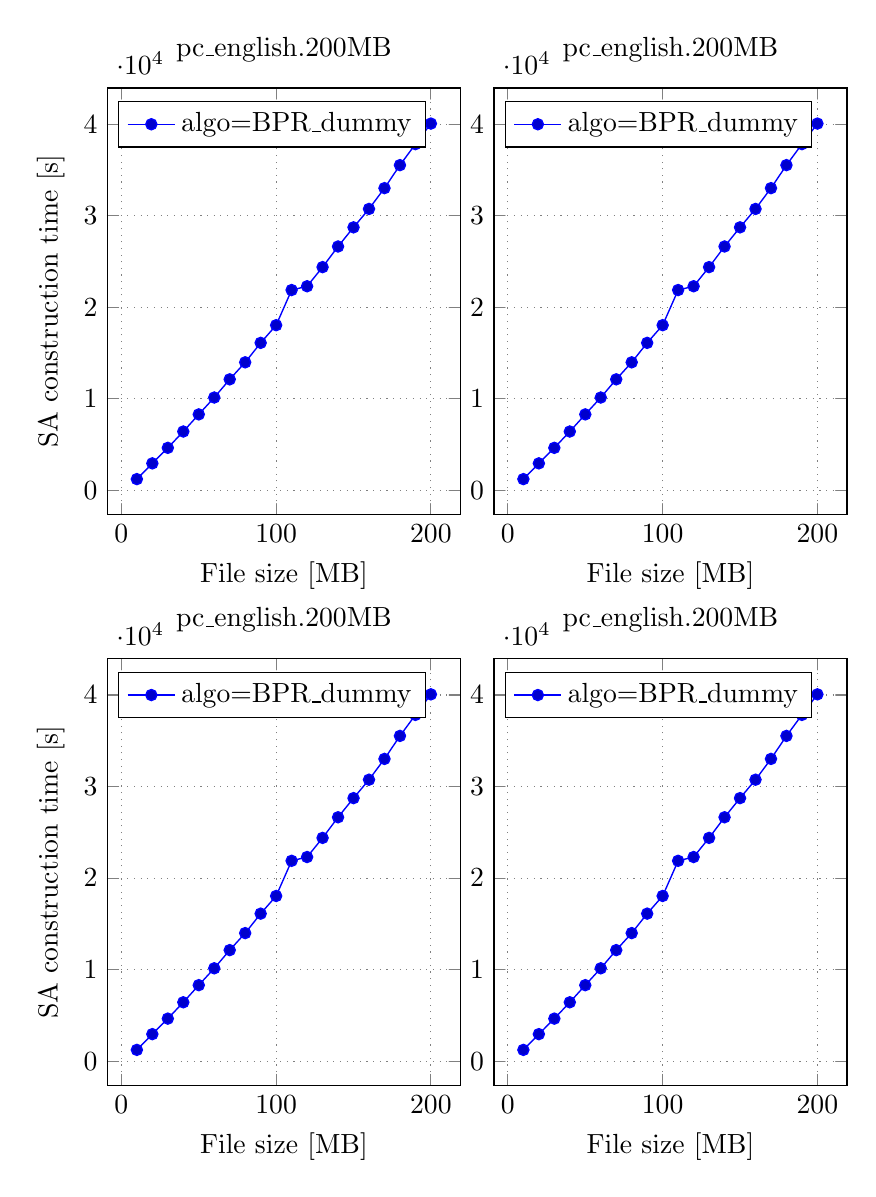
\begin{tikzpicture}
        \begin{axis}[
                name=axis1,
                width=0.5\textwidth,
                height=70mm,
                title={pc\_english.200MB},
                xlabel={File size [MB]},
                ylabel={SA construction time [s]},
            ]

            %% MULTIPLOT(algo) SELECT prefix/1000000 AS x, time AS y, MULTIPLOT
            %% FROM stats WHERE algo="BPR_dummy" GROUP BY MULTIPLOT,x ORDER BY MULTIPLOT,x
            \addplot coordinates { (10,1234.0) (20,2954.0) (30,4649.0) (40,6433.0) (50,8303.0) (60,10145.0) (70,12131.0) (80,13990.0) (90,16116.0) (100,18045.0) (110,21886.0) (120,22299.0) (130,24388.0) (140,26642.0) (150,28733.0) (160,30743.0) (170,33016.0) (180,35528.0) (190,37823.0) (200,40068.0) };
            \addlegendentry{algo=BPR\_dummy};

        \end{axis}
        \begin{axis}[
                at={(axis1.outer north east)},
                anchor=outer north west,
                name=axis2,
                width=0.5\textwidth,
                height=70mm,
                title={pc\_english.200MB},
                xlabel={File size [MB]},
            ]

            %% MULTIPLOT(algo) SELECT prefix/1000000 AS x, time AS y, MULTIPLOT
            %% FROM stats WHERE algo="BPR_dummy" GROUP BY MULTIPLOT,x ORDER BY MULTIPLOT,x
            \addplot coordinates { (10,1234.0) (20,2954.0) (30,4649.0) (40,6433.0) (50,8303.0) (60,10145.0) (70,12131.0) (80,13990.0) (90,16116.0) (100,18045.0) (110,21886.0) (120,22299.0) (130,24388.0) (140,26642.0) (150,28733.0) (160,30743.0) (170,33016.0) (180,35528.0) (190,37823.0) (200,40068.0) };
            \addlegendentry{algo=BPR\_dummy};

        \end{axis}
        \begin{axis}[
                at={(axis1.outer south west)},
                anchor=outer north west,
                name=axis3,
                width=0.5\textwidth,
                height=70mm,
                title={pc\_english.200MB},
                xlabel={File size [MB]},
                ylabel={SA construction time [s]},
            ]

            %% MULTIPLOT(algo) SELECT prefix/1000000 AS x, time AS y, MULTIPLOT
            %% FROM stats WHERE algo="BPR_dummy" GROUP BY MULTIPLOT,x ORDER BY MULTIPLOT,x
            \addplot coordinates { (10,1234.0) (20,2954.0) (30,4649.0) (40,6433.0) (50,8303.0) (60,10145.0) (70,12131.0) (80,13990.0) (90,16116.0) (100,18045.0) (110,21886.0) (120,22299.0) (130,24388.0) (140,26642.0) (150,28733.0) (160,30743.0) (170,33016.0) (180,35528.0) (190,37823.0) (200,40068.0) };
            \addlegendentry{algo=BPR\_dummy};

        \end{axis}
        \begin{axis}[
                at={(axis3.outer north east)},
                anchor=outer north west,
                name=axis4,
                width=0.5\textwidth,
                height=70mm,
                title={pc\_english.200MB},
                xlabel={File size [MB]},
            ]

            %% MULTIPLOT(algo) SELECT prefix/1000000 AS x, time AS y, MULTIPLOT
            %% FROM stats WHERE algo="BPR_dummy" GROUP BY MULTIPLOT,x ORDER BY MULTIPLOT,x
            \addplot coordinates { (10,1234.0) (20,2954.0) (30,4649.0) (40,6433.0) (50,8303.0) (60,10145.0) (70,12131.0) (80,13990.0) (90,16116.0) (100,18045.0) (110,21886.0) (120,22299.0) (130,24388.0) (140,26642.0) (150,28733.0) (160,30743.0) (170,33016.0) (180,35528.0) (190,37823.0) (200,40068.0) };
            \addlegendentry{algo=BPR\_dummy};

        \end{axis}
    \end{tikzpicture}
\end{center}

\section{Extra memory usage}
\begin{center}
    \begin{tikzpicture}
        \begin{axis}[
                title={pc\_english.200MB},
                xlabel={File Size [Bytes]},
                ylabel={Extra Memory [Bytes]},
            ]

            %% MULTIPLOT(algo) SELECT prefix AS x, memPeak AS y, MULTIPLOT
            %% FROM stats WHERE algo="BPR_dummy" GROUP BY MULTIPLOT,x ORDER BY MULTIPLOT,x
            \addplot coordinates { (10000000,10000000) (1e+08,1e+08) (1.1e+08,1.1e+08) (1.2e+08,1.2e+08) (1.3e+08,1.3e+08) (1.4e+08,1.4e+08) (1.5e+08,1.5e+08) (1.6e+08,1.6e+08) (1.7e+08,1.7e+08) (1.8e+08,1.8e+08) (1.9e+08,1.9e+08) (20000000,20000000) (2e+08,2e+08) (30000000,30000000) (40000000,40000000) (50000000,50000000) (60000000,60000000) (70000000,70000000) (80000000,80000000) (90000000,90000000) };
            \addlegendentry{algo=BPR\_dummy};

        \end{axis}
    \end{tikzpicture}
\end{center}

\section{Extra memory per input byte}
\begin{center}
    \begin{tikzpicture}
        \begin{axis}[
                title={pc\_english.200MB},
                xlabel={File Size [MB]},
                ylabel={Extra Memory in Bytes per input Byte},
            ]

            %% MULTIPLOT(algo) SELECT prefix/1000000 AS x, memPeak/prefix AS y, MULTIPLOT
            %% FROM stats WHERE algo="BPR_dummy" GROUP BY MULTIPLOT,x ORDER BY MULTIPLOT,x
            \addplot coordinates { (10,1) (20,1) (30,1) (40,1) (50,1) (60,1) (70,1) (80,1) (90,1) (100,1) (110,1) (120,1) (130,1) (140,1) (150,1) (160,1) (170,1) (180,1) (190,1) (200,1) };
            \addlegendentry{algo=BPR\_dummy};

        \end{axis}
    \end{tikzpicture}
\end{center}

\end{document}

